\documentclass[12pt]{report}
\usepackage[utf8x]{inputenc}
\usepackage{graphicx}
\usepackage{gensymb}
\usepackage{algorithm}
\usepackage[noend]{algpseudocode}
\usepackage{algpseudocode}
\graphicspath{ {./images/} }
\usepackage{fancyhdr}


\title{ETERNITY: FUNCTIONS}								
\author{Surya Prakash Govindaraju}						
\date{}

\makeatletter
\let\thetitle\@title
\let\theauthor\@author
\let\thedate\@date
\makeatother

\pagestyle{fancy}
\fancyhf{}
\rhead{\thetitle}
\cfoot{\thepage}

\begin{document}

\begin{titlepage}
	\centering
    \vspace*{0.5 cm}
\begin{center}    \textsc{\Large Concordia University}\\[2.0 cm]	\end{center}
	\textsc{\Large  SOEN 6011 - Software Engineering Process }\\[0.5 cm]
	\rule{\linewidth}{0.2 mm} \\[0.4 cm]
	{ \huge \textbf \thetitle}\\[0.2 cm]
	{ \huge \textbf{arccos(x)}}
	\rule{\linewidth}{0.2 mm} \\[1.5 cm]

\begin{center}   {\Large Deliverable 1}\\[2.0 cm]
\end{center}	
\begin{center}   {\Large \textbf{\theauthor}} \\[0.2 cm]
                 {\large Student ID : 40085527 }\\[0.2 cm]
                 {\large Team D }\\[2.0 cm]	
                 {\large https://github.com/Surya64/SOEN-6011}
\end{center}
	
\end{titlepage}

\tableofcontents
\pagebreak

\renewcommand{\thesection}{\arabic{section}}
\section{Introduction}
\subsection{Description}
The arccos function is the inverse of the cosine function. It returns the angle whose cosine is a given number. The angle returned by this function is measured in radians or in degrees.The inverse is also called as acos or $cos^{-1}$.

\begin{figure}[h!]
\begin{center}
  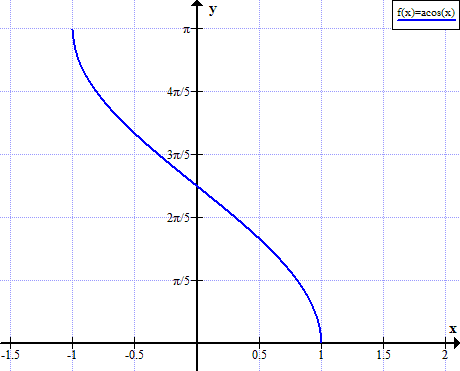
\includegraphics[width=6cm, height=5.2cm]{arccos-graph.png}
  \end{center}
  \caption{Graph of inverse cosine function (Source: Google Images)}
\end{figure}

arccos function is useful when trying to determine the remaining two angles of a right triangle when the length of sides is known. It is calculated as below

$$\theta = arccos( \frac{adjacent}{hypotenuse})$$

Derivative of arccos is given by,

$$ \frac{d}{dx} arccos(x) = \frac{-1}{\sqrt{1-x^2}} $$

\subsection{Domain}
  $$−1 \leq x \leq 1 $$
\subsection{Co-Domain}  
$$0 \leq y \leq \pi  $$ 
\begin{center}
 or   
\end{center}
$$0^\circ\leq y \leq 180^\circ $$

\subsection{Characteristic}
\begin{itemize}
    \item Function is neither even nor odd
    \item Function is decreasing
    \item Ranges of the inverse function are subsets of the domain
    \item Function is defined for complex arguments
    \item Function is multi-valued, unless its principal value is defined
\end{itemize}

\newpage
\section{Functional Requirement}
\subsection{Assumptions}
\begin{itemize}
\item ID: A1
\begin{itemize}
\item Description: Input for the function arccos(x) is real number
\end{itemize}
\item ID: A2
\begin{itemize}
\item Description: Output of the function arccos(x) is in radians\degree
\end{itemize}
\item ID: A3
\begin{itemize}
\item Description: For values out of range, the result is undefined and throws error
\end{itemize}
\item ID: A4
\begin{itemize}
\item Description: The results obtained from approximation formulas will have some relative error.
\end{itemize}
\end{itemize}


\subsection{Requirements}
\begin{itemize}
\item ID: R1
\begin{itemize}
\item Version:  1.0
\item Type: Functional Requirement
\item Priority: 1
\item Risk: High
\item Description: For any other input out of domain, the system should throw error
\item Rationale: Output is not defined for values out of domain range
\end{itemize}
\item ID: R2
\begin{itemize}
\item Version:  1.0
\item Type: Functional Requirement
\item Priority: 1
\item Risk: High
\item Description: There is no duplicate output value for an input within domain range
\item Rationale: one to one mapping between the domain and co domain
\end{itemize}
\item ID: R3
\begin{itemize}
\item Version:  1.0
\item Type: Functional Requirement
\item Priority: 1
\item Risk: High
\item Description: For valid input, the output is displayed in degree or radians
\item Rationale: Output is defined with in co domain range.
\end{itemize}
\item ID: R4
\begin{itemize}
\item Version:  1.0
\item Type: Functional Requirement
\item Priority: 2
\item Risk: medium
\item Description: User provides only one input value for the function
\item Rationale: x is the input for arccos
\end{itemize}
\item ID: R5
\begin{itemize}
\item Version:  1.0
\item Type: Non- Functional Requirement
\item Priority: 3
\item Risk: Low
\item Description: The calculation of the function should be completed within a desired time window
\item Rationale: To have a better performance
\end{itemize}
\end{itemize}


 
\newpage
\section{Algorithm}
\begin{algorithm}
\caption{Approximation algorithm for StrictMath}
\begin{algorithmic}[1]
\If{$x$ is negative}
  \State $x = -x$
\EndIf
\If{$x$ is equal to 1}
  \State \textbf{return} $negative$ $? PI : 0$
\EndIf
\If{$x$ is less than 0.5}
  \If{$x$ less than $\frac{1}{K}$}
  \State \textbf{return} $\frac{PI}{2}$
  \EndIf
\State z = $ x * x $
\State p = $ z * (P0 + z * (P1 + z * (P2 + z * (P3 + z * (P4 + z * P5)))))$
\State $q = 1 + z * (Q1 + z * (Q2 + z * (Q3 + z * Q4)))$
\State $r = x - (PI_L / 2 - x * (p / q))$
  \State \textbf{return} $negative ? \frac {PI}{2 + r} :\frac {PI}{2 - r}$
\EndIf
\If{$x$ is negative}
\State z = $(1 + x) * 0.5$
\State p = $ z * (P0 + z * (P1 + z * (P2 + z * (P3 + z * (P4 + z * P5)))))$
\State $q = 1 + z * (Q1 + z * (Q2 + z * (Q3 + z * Q4)))$
\State s = $sqrt(z)$
\State w = $\frac{p }{ q }* s - \frac{PI_L}{2}$
  \State \textbf{return} $PI - 2 * (s + w)$
\State $z = (1 - x) * 0.5$
\State $s = sqrt(z)$
\State $df = (float) s$
\State $c = (z - df * df) / (s + df)$
\State p = $ z * (P0 + z * (P1 + z * (P2 + z * (P3 + z * (P4 + z * P5)))))$
\State $q = 1 + z * (Q1 + z * (Q2 + z * (Q3 + z * Q4)))$
\State $w = p / q * s + c$
\State \textbf{return} $2 * (df + w)$
\EndIf

\end{algorithmic}
\end{algorithm}

\pagebreak
\begin{algorithm}
\caption{polynomial approximation algorithm using arctan}
\begin{algorithmic}[1]
\If{$x$ is negative}
  \State $arctan(-x) = -arctan(x)$
\EndIf
\If{$x$ is greater than 1}
  \State \textbf{return} $arctan(x) = \frac{\pi}{2}-arctan(\frac{1}{x})$ \Comment{To replace value bigger than 1}
\EndIf
\If{$x > 2-\sqrt{3}$}
  \State \textbf{return} $arctan(x) =\frac{\pi}{6}+arctan(\frac{\sqrt{3}x-1}{\sqrt{3}+x})$ \Comment{To replace value bigger than $2-\sqrt{3}$}
\EndIf
\State $arctan(x) = x - \frac{x^3}{3} + \frac{x^5}{5}$
\State Substitute the $arctan(x)$ value in step 6
\State Results is in radians, convert by multiplying by $\frac{180}{\pi} $
\end{algorithmic}
\end{algorithm}

\subsection{Description}
For calculating the inverse cosine of a value, above are the two approximation algorithms selected. Algorithm1 focus on the approximation that is derived from the Strict Math which basically focuses on constant variables used in the approximation. The algorithm also uses the square root function and the value of pi is declared as a constant variable. The results obtained are in radians and is a approximation value for arccos trigonometric function.
\paragraph{}
Algorithm2 is a polynomial approximation algorithm which is used to calculate the arccos function using the arctan function. From the Taylor's series of arctan(x), the value of arctan is calculated and obtained the result. The results are in radians and converted to degree by multiplying with $\frac{180}{\pi}$.

\subsection{Advantages and Disadvantages}
\textbf{Advantages}
\begin{itemize}
    \item Algorithm1 is provides the more accurate results for the value of x with in the domain
    \item Algorithm1 uses no other trigonometric function which will have no dependencies
    \item Performance is faster in algorithm1 than algorithm2 as estimated from the Big O Notation
\end{itemize}

\textbf{Disadvantages}
\begin{itemize}
    \item For algorithm2, the higher order derivative of inverse trigonometric function becomes extremely complicated
    \item Algorithm2 approximation is only for small arguments and provides no accurate results for large arguments
\end{itemize}

\begin{thebibliography}{9}
\bibitem{mathonweb}
Mathonweb,
\\\texttt{http://mathonweb.com/help\_ebook/html/algorithms.htm\#arcsin}

\bibitem{Wolframweb} 
Wolfram,
\\\texttt{https://reference.wolfram.com/language/ref/ArcCos.html}

\bibitem{wiki} 
Wikipedia,
\\\texttt{https://en.wikipedia.org/wiki/Taylor\_series}

\bibitem{rapidtableswebsite}
RapidTables,
\\\texttt{https://www.rapidtables.com/math/trigonometry/arccos.html}
\end{thebibliography}
\end{document}
